\subsection{M.PD.13 - Linee medie di codice per metodo}

\begin{figure}[H]
  \centering
  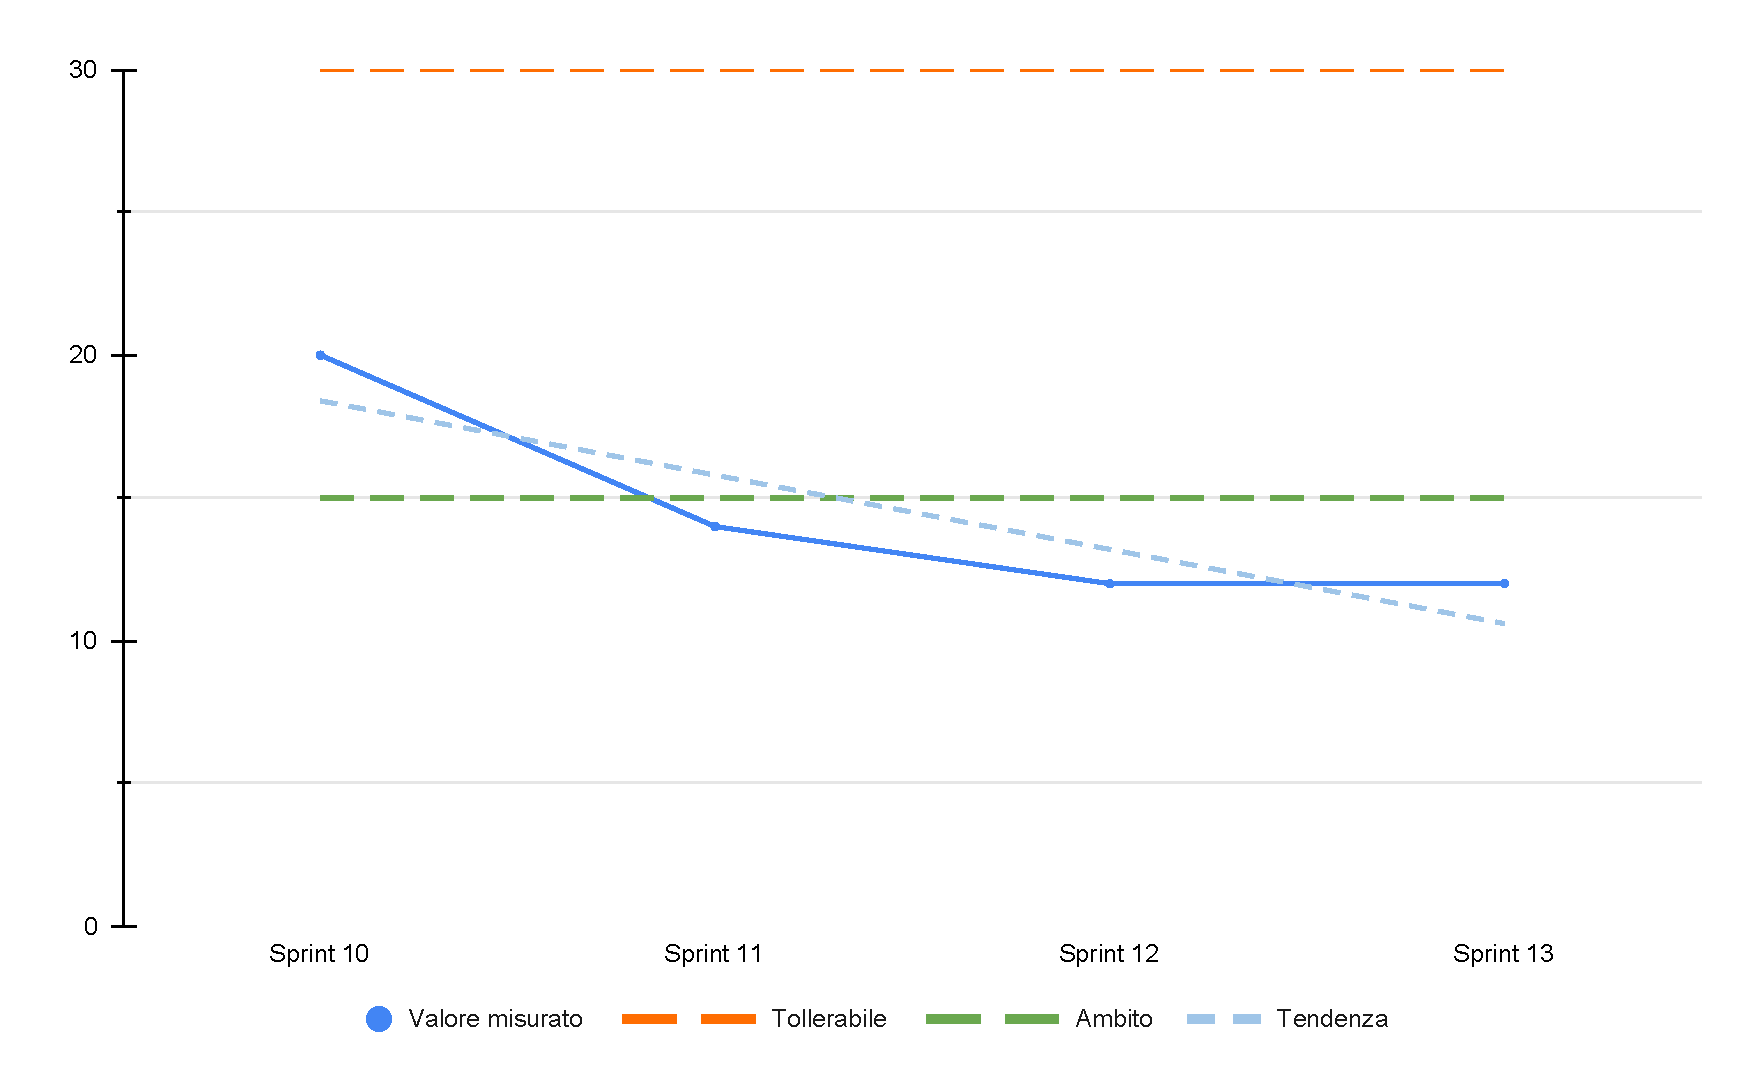
\includegraphics[width=\textwidth]{assets/linee_medie_codice.pdf}
  \caption{M.PD.13 - Linee medie di codice per metodo}
\end{figure}

\par Inizialmente, il numero medio di linee di codice per metodo (o funzione) non ha raggiunto la soglia ambita, rimanendo all'interno del range considerato accettabile. Questo risultato è stato influenzato dalla necessità di una fase di studio preliminare per la separazione delle responsabilità dei componenti e per l'implementazione del modello architetturale scelto. Inoltre, il codice del \glossario{front-end} era caratterizzato da ridondanze e mancava di una struttura chiara. A partire dall'undicesimo \glossario{sprint}, il team ha eseguito un refactoring completo del codice front-end, suddividendo le funzioni più complesse in segmenti più piccoli e gestibili. A seguire, l'implementazione dell'architettura \glossario{back-end} ha permesso una chiara separazione delle responsabilità tra i vari metodi. Come mostrato nel grafico, queste modifiche progettuali hanno consentito al team di raggiungere e superare la soglia ambita.